\section{Neuronová síť}
Neuronová síť je výpočetní model, který je inspirován fungováním lidského mozku.
Neuronová sít se skláda z neuronů a váh.
Neurony jsou propojeny váhami mezi vrstvami.
Každá neurovová síť má vstupní, skryté a výstupní vrstvy.
Počty neuronů v každé vrstvě závisí na konkrétním využití a na problému, který má neuronová síť řešit.

Každý neuron představuje jednoduchý výpočetní prvek, který zpravová vstupy a generuje výstup.
Vstupy a výstupy jsou spojeny váhami, které ovlivňují hodnoty neuronů, ze kterých váha vede.
Dále má každý neuron svůj bias, který ovlivňuje jeho hodnotu.

Existují různé typy neuronových sítí, které se liší tím, jak se neurony mezi vrstvami propojují.
Mezi nejběžnější typy patří neuronové sítě typu perceptrony, vícevrstvé perceptory, konvulační neuronové sítě a rekurentní neuronové sítě.

\subsection{Fungování neuronových sítí}
Neuronová síť načte vstup a hodnoty projdou celou síťí.
Až hodnoty projdou celou sítí nakonec, ve výstupní vrstvě je výsledek.

Hodnota konkrétního neuronu se spočítá tak, že se sečte hodnota všech neuronů vynásobena spojující váhou, přičte se bias daného neuronu a zavolá se nějaká aktivační funkce.
Aktivačních funkcí je řada. Mezi nejběžnější patří například sigmoid nebo ReLU. Výběr ideální aktivační funkce opět zavisí na problému, který síť řeší.
Tyto funkce v jednoduchosti transformují vstupy neuronu na jeho výstupy.
Aktivační funkce dodávají sítím jistou nelinearitu, která umožňuje sítím řešit i problémy, které nejsou linearní.

\begin{figure}[h]
    \centering
    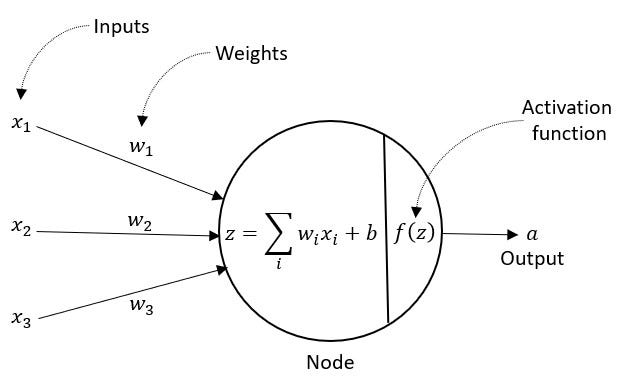
\includegraphics[width=0.25\textwidth]{images/neuron.jpg}
    \caption{Umělý neuron}
    \cite{umely_neuron}
\end{figure}


